\documentclass{beamer}
\mode<presentation> {
\usepackage{color}
\definecolor{bottomcolour}{rgb}{0.21,0.11,0.21}
\definecolor{middlecolour}{rgb}{0.21,0.11,0.21}
\setbeamercolor{structure}{fg=white}
\setbeamertemplate{frametitle}[default]%[center]
\setbeamercolor{normal text}{bg=black, fg=white}
\setbeamertemplate{background canvas}[vertical shading]
[bottom=bottomcolour, middle=middlecolour, top=black]
\setbeamertemplate{items}[circle]
\setbeamertemplate{navigation symbols}{} %no nav symbols
\setbeamercolor{block title}{use=structure,fg=white,bg=structure.fg!50!red!50!blue!100!green}
\setbeamercolor{block body}{parent=normal text,use=block title,bg=block title.bg!5!white!10!bg,fg=white}
\setbeamertemplate{navigation symbols}{}
\newcounter{moncompteur}
}
\usepackage{graphicx} 
\usepackage{booktabs} 
\usepackage[utf8]{inputenc}  
\usepackage[T1]{fontenc}  
\usepackage{geometry}     
%\usepackage[francais]{babel} 
\usepackage{eurosym}
\usepackage{verbatim}
\usepackage{ragged2e}
\justifying
%%%%%%%%%%%%%%%%%%%%%%%%%%%%%%%%%%%%%%%%%%%%%%%%%%%%%%%%%%%%%%%%
%% ccBeamer 0.1, 2007-07-02                                   %%
%% Written by Sebastian Pipping <webmaster@hartwork.org>      %%
%% ---------------------------------------------------------- %%
%% Licensed under Creative Commons Attribution-ShareAlike 3.0 %%
%% http://creativecommons.org/licenses/by-sa/3.0/             %%
%%%%%%%%%%%%%%%%%%%%%%%%%%%%%%%%%%%%%%%%%%%%%%%%%%%%%%%%%%%%%%%%


%% Images
\newcommand{\CcImageBy}[1]{%
	
\includegraphics[scale=#1]{creative_commons/cc_by_30.pdf}%
}
\newcommand{\CcImageCc}[1]{%
	
\includegraphics[scale=#1]{creative_commons/cc_cc_30.pdf}%
}
\newcommand{\CcImageDevNations}[1]{%
	
\includegraphics[scale=#1]{creative_commons/cc_dev_nations_30.pdf}%
}
\newcommand{\CcImageNc}[1]{%
	
\includegraphics[scale=#1]{creative_commons/cc_nc_30.pdf}%
}
\newcommand{\CcImageNd}[1]{%
	
\includegraphics[scale=#1]{creative_commons/cc_nd_30.pdf}%
}
\newcommand{\CcImagePd}[1]{%
	
\includegraphics[scale=#1]{creative_commons/cc_pd_30.pdf}%
}
\newcommand{\CcImageSa}[1]{%
	
\includegraphics[scale=#1]{creative_commons/cc_sa_30.pdf}%
}
\newcommand{\CcImageSampling}[1]{%
	
\includegraphics[scale=#1]{creative_commons/cc_sampling_30.pdf}%
}
\newcommand{\CcImageSamplingPlus}[1]{%
	
\includegraphics[scale=#1]{creative_commons/cc_sampling_plus_30.pdf}%
}


%% Groups
\newcommand{\CcGroupBy}[1]{% zoom
	\CcImageBy{#1}%
}
\newcommand{\CcGroupByNc}[2]{% zoom, gap
	\CcImageBy{#1}\hspace*{#2}\CcImageNc{#1}%
}
\newcommand{\CcGroupByNcNd}[2]{% zoom, gap
	\CcImageBy{#1}\hspace*{#2}\CcImageNc{#1}\hspace*{#2}\CcImageNd{#1}%
}
\newcommand{\CcGroupByNcSa}[2]{% zoom, gap
	\CcImageBy{#1}\hspace*{#2}\CcImageNc{#1}\hspace*{#2}\CcImageSa{#1}%
}
\newcommand{\CcGroupByNd}[2]{% zoom, gap
	\CcImageBy{#1}\hspace*{#2}\CcImageNd{#1}%
}
\newcommand{\CcGroupBySa}[2]{% zoom, gap
	\CcImageBy{#1}\hspace*{#2}\CcImageSa{#1}%
}
\newcommand{\CcGroupDevNations}[1]{% zoom
	\CcImageDevNations{#1}%
}
\newcommand{\CcGroupNcSampling}[2]{% zoom, gap
	\CcImageNc{#1}\hspace*{#2}\CcImageSampling{#1}%
}
\newcommand{\CcGroupPd}[1]{% zoom
	\CcImagePd{#1}%
}
\newcommand{\CcGroupSampling}[1]{% zoom
	\CcImageSampling{#1}%
}
\newcommand{\CcGroupSamplingPlus}[1]{% zoom
	\CcImageSamplingPlus{#1}%
}


%% Text
\newcommand{\CcLongnameBy}{Attribution}
\newcommand{\CcLongnameByNc}{Attribution-NonCommercial}
\newcommand{\CcLongnameByNcNd}{Attribution-NoDerivs}
\newcommand{\CcLongnameByNcSa}{Attribution-NonCommercial-ShareAlike}
\newcommand{\CcLongnameByNd}{Attribution-NoDerivs}
\newcommand{\CcLongnameBySa}{Attribution-ShareAlike}

\newcommand{\CcNote}[1]{% longname
	This work is licensed under the \textit{Creative Commons #1 3.0 License}.%
}

\title[Sécurité et vie privée : démystifions les dangers d'Internet !]{Sécurité et vie privée \\~\\ Démystifions les dangers d'Internet !}
\author{Genma}
%========================================
\begin{document}
%% Titlepage
\begin{frame}
	\titlepage
	\vfill
	\begin{center}
		\CcGroupByNcSa{0.83}{0.95ex}\\[2.5ex]
		{\tiny\CcNote{\CcLongnameByNcSa}}
		\vspace*{-2.5ex}
	\end{center}
\end{frame}

%--------------------------------------------------------------------------------
\begin{frame}
\frametitle{Accessibilité}

\begin{block}{Visuelle}
\justifying{
\begin{itemize}
\item Est-ce que tout le monde arrive à lire la présentation ?
\item Elle est disponible en ligne, pas la peine de prendre de notes :-)
\end{itemize}}
\end{block}
\begin{center}

\includegraphics[scale=0.4]{./images/accessibilite_v2.jpg}
\end{center}

\begin{block}{Auditive}
\begin{itemize}
\justifying{
\item Je parle vite. Très vite.
\item Merci de me faire signe pour me demander de ralentir, d'articuler.
}
\end{itemize}
\end{block}
\end{frame}

%--------------------------------------------------------------------------------
\begin{frame}
\frametitle{
\includegraphics[scale=0.4]{./images/Genma.jpg} \ \ \  À propos de Genma  }
\begin{columns}[c] 
\column{.55\textwidth} 
\textbf{Où me trouver sur Internet?}
\begin{itemize}
\item Le Blog de Genma : \url{https://blog.genma.fr}
\item Twitter : \url{https://twitter.com/genma}
\end{itemize}
\column{.5\textwidth} 
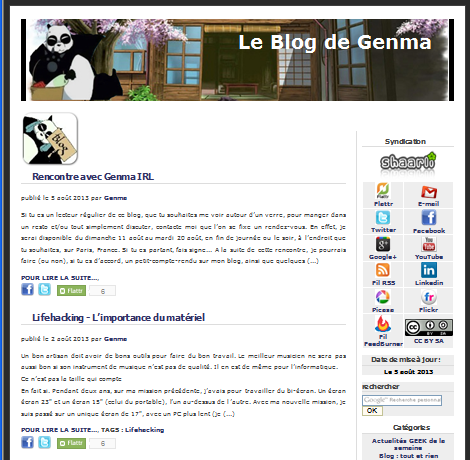
\includegraphics[scale=0.40] {./images/blog.png} 
\end{columns}
\end{frame}

%----------------------------------------------------------------------------------------
\begin{frame}
\frametitle{De quoi allons-nous parler? }
Deux parties :
\begin{itemize}
\justifying{
\item Hygiène numérique et des règles de bases
\item Vie privée sur Internet \& données personnelles 
}
\end{itemize}
\end{frame}

%========================================================================================
\begin{frame}
\begin{center}
\Huge{Un peu d'hygiène numérique}
\\~\\
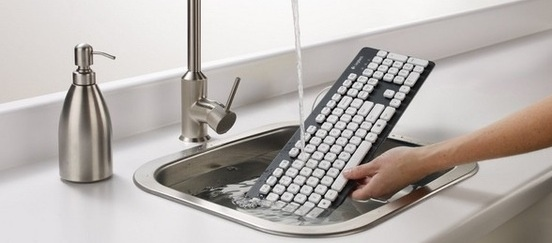
\includegraphics[scale=0.5]{./images/nettoyer_son_clavier.jpg}
\end{center}
\end{frame}

%----------------------------------------------------------------------------------------
\begin{frame}
\frametitle{L'hygiène numérique?}
\begin{block}{Une définition?}
\justifying{
L'hygiène est un ensemble de mesures destinées à prévenir les infections et l'apparition de maladies infectieuses.
\\
L'hygiène numérique, ce sont des règles destinées à mieux utiliser son ordinateur, en sécurité, de façon simple.
}
\end{block}
\emph{L'hygiène numérique c'est comment éviter la gastro-informatique.}
\end{frame}

%----------------------------------------------------------------------------------------
\begin{frame}
\frametitle{Un exemple}
\begin{block}{On me vole mon PC}
\justifying{
\begin{itemize}
\item  Quelles sont les données que je perds ? Amène la notion de \emph{sauvegarde}.
\item  Quelles sont les données que l'on trouve ? Amène la notion de \emph{chiffrement, de coffre-fort numérique}.
\end{itemize}
}
\end{block}
\begin{center}
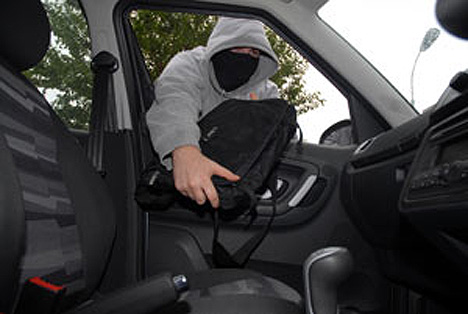
\includegraphics[scale=0.5] {./images/laptopthief.jpg}
\end{center}
\end{frame}

%----------------------------------------------------------------------------------------
\begin{frame}
\frametitle{Sauvegarde simple et efficace}

\begin{block}{Le disque dur externe}
\begin{itemize}
\justifying{
\item Méthode simple : copier-coller.
\item Méthode plus avancé : on "synchronise".
\item On le dépose chez un ami, un voisin, un parent (pour éviter le vol, l'incendie...)
}
\end{itemize}
Petit plus : chiffrer le disque pour plus de confidentialité.
\end{block}
\begin{center}
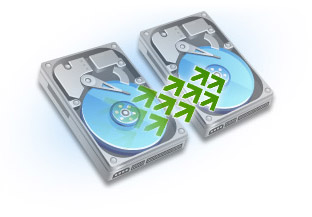
\includegraphics[scale=0.5] {./images/backup.jpg}
\end{center}
\end{frame}

%-----------------------------------------------
\begin{frame}
\frametitle{Coffre-fort numérique ? Veracrypt}
\begin{center}
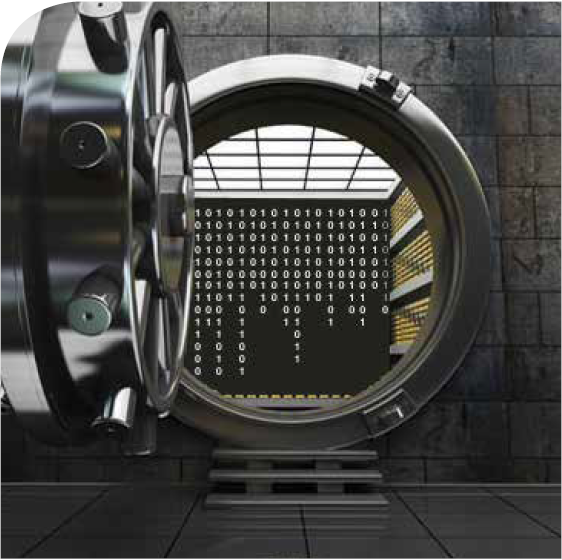
\includegraphics[scale=0.5]{./images/coffre_fort_numerique.png}
\end{center}
\end{frame}

%-----------------------------------------------
\begin{frame}
\frametitle{Coffre-fort numérique ? Veracrypt}
\begin{center}
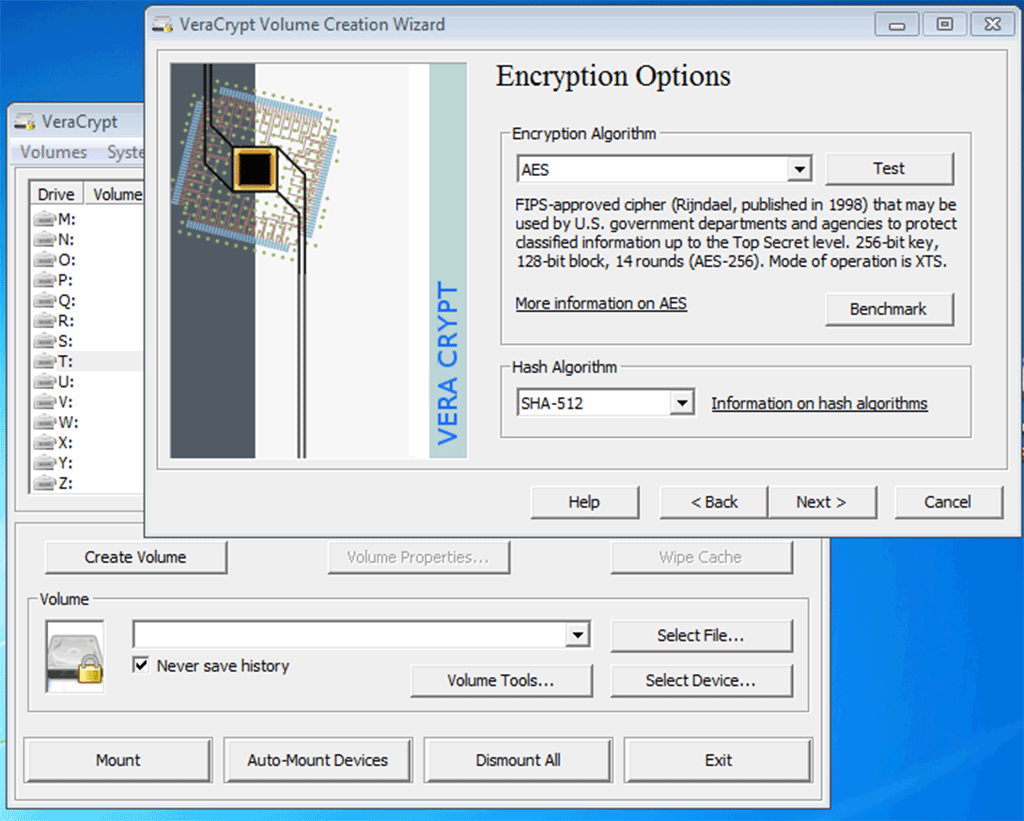
\includegraphics[scale=0.3]{./images/vercrypt.png}
\end{center}
\end{frame}

%-----------------------------------------------
\begin{frame}
\frametitle{Crypté ? Cryptage ?}
\begin{center}
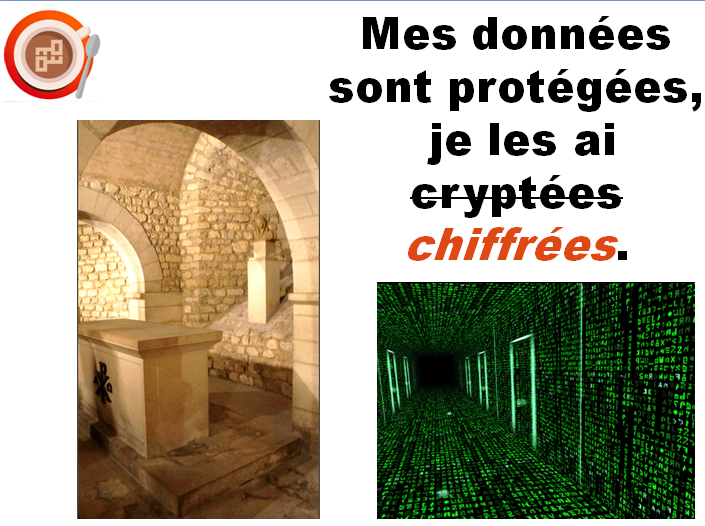
\includegraphics[scale=0.5]{./images/chiffrees_vs_cryptees.png}
\end{center}
\end{frame}

%----------------------------------------------------------------------------------------
\begin{frame}
\Huge{\centerline{Les mots de passe}}

\begin{center}
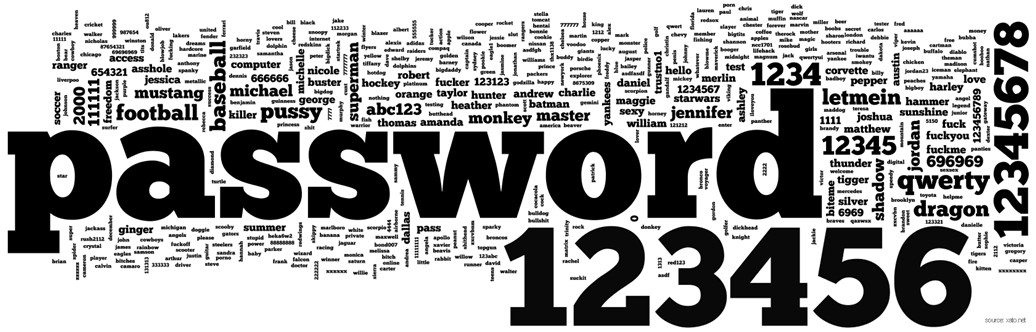
\includegraphics[scale=0.6] {./images/password.png}
\end{center}
\end{frame}

%----------------------------------------------------------------------------------------
\begin{frame}
\frametitle{Les mots de passe}
\begin{block}{Règles}
\begin{itemize}
\justifying{
\item Plus c'est long, plus c'est bon
\item Ne pas avoir le même mot de passe pour deux comptes en ligne.
\item Passer à des \emph{phrases de passe} (technique des dés...)
}
\end{itemize}
\end{block}
\begin{block}{Trop de mot de passe à retenir?}
Il y a le logiciel KeepassX.
\end{block}
\end{frame}

%-----------------------------------------------
\begin{frame}
\frametitle{KeepassX, le coffre-fort numérique des mots de passe}
\begin{center}
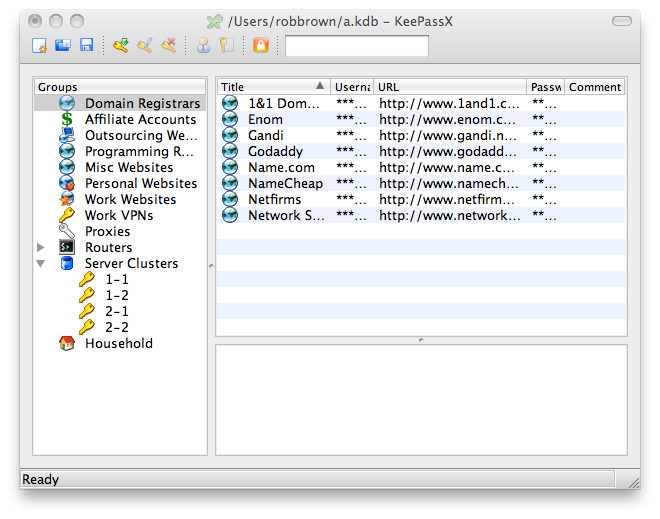
\includegraphics[scale=0.5]{./images/keypassX.png}
\end{center}
\end{frame}

%----------------------------------------------------------------------------------------
\begin{frame}
\frametitle{Les mots de passe}
\begin{block}{Les sites permettant de tester ses mots de passes?}
\begin{itemize}
\justifying{
\item Ils sont la meilleure façon de constituer une base de données de mots de passe.
\item Ne pas tester son vrai mot de passe mais un mot de passe du même type/de la même forme.
\item Les mots de passe sont personnels 
}
\end{itemize}
\end{block}

\begin{block}{Parents - enfants}
\justifying{
Tant qu’on est mineur on doit les donner à ses parents. Les parents qui sont des gens bien et responsables, ne sont pas là pour les utiliser pour espionner leurs enfants mais seulement au cas où.}
\end{block}
\end{frame}
%----------------------------------------------------------------------------------------
\begin{frame}
\frametitle{Gestion des comptes}
\begin{block}{Des comptes pour des usages différents}
\begin{itemize}
\justifying{
\item Créer un compte utilisateur et un compte administrateur.
\item Au quotidien, utiliser le compte utilisateur.
\item Le compte administrateur porte bien son nom, il ne doit servir qu'aux tâches d'administration (installation des logiciels...)
}
\end{itemize}
\justifying{
Quand l'ordinateur pose une question "Je dois lancer ce programme", réfléchir. Ne pas dire oui tout de suite.
}
\end{block}
\end{frame}

%----------------------------------------------------------------------------------------
\begin{frame}
\frametitle{Mises à jour de sécurité}
\justifying{
\begin{block}{FAIRE LES MISES A JOUR}
\begin{itemize}
\item Avoir un système à jour.
\item Avoir des logiciels à jour.
\item Avoir un antivirus à jour.
\end{itemize}
\end{block}
}

\begin{block}{Les logiciels ont des bugs}
\begin{itemize}
\justifying{
\item Un bug peut-être utilisé par un virus...
 \item Mettre à jour, c'est corriger les bugs, donc se protéger.
}\end{itemize}
\end{block}
\end{frame}
%----------------------------------------------------------------------------------------
\begin{frame}
\frametitle{Mises à jour de sécurité}
\begin{center}
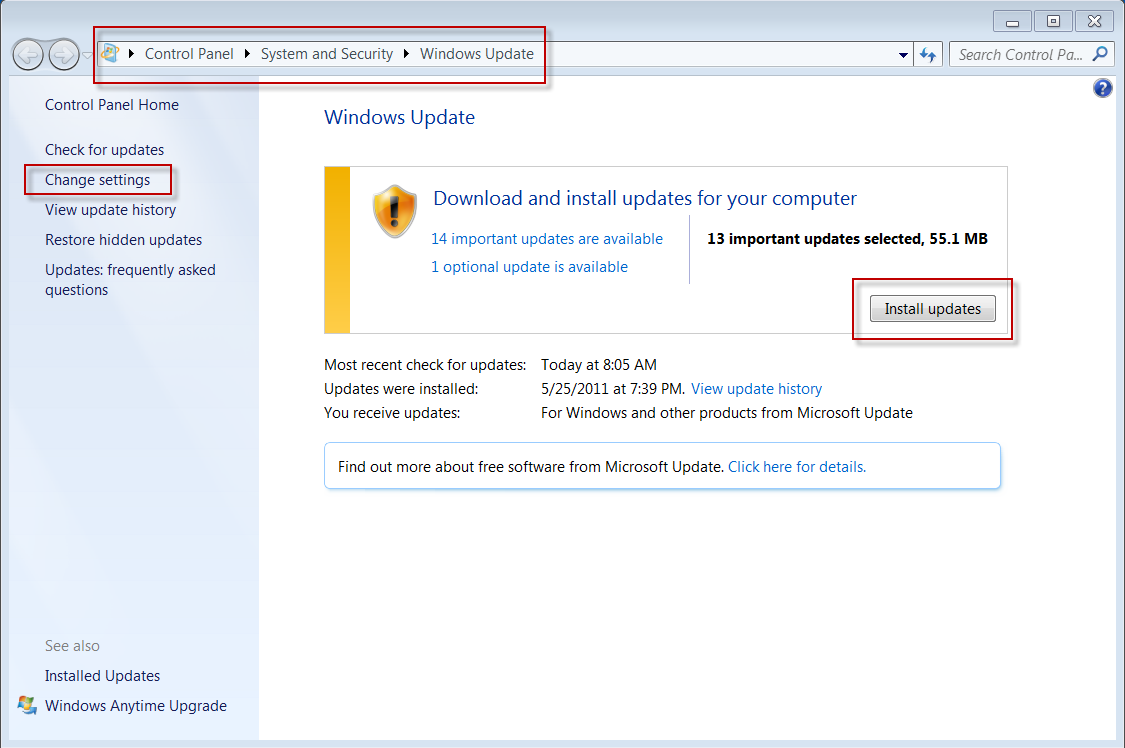
\includegraphics[scale=0.5] {./images/Maj01.png}
\end{center}
\end{frame}
\begin{frame}
\frametitle{ Mises à jour de sécurité}
\begin{center}
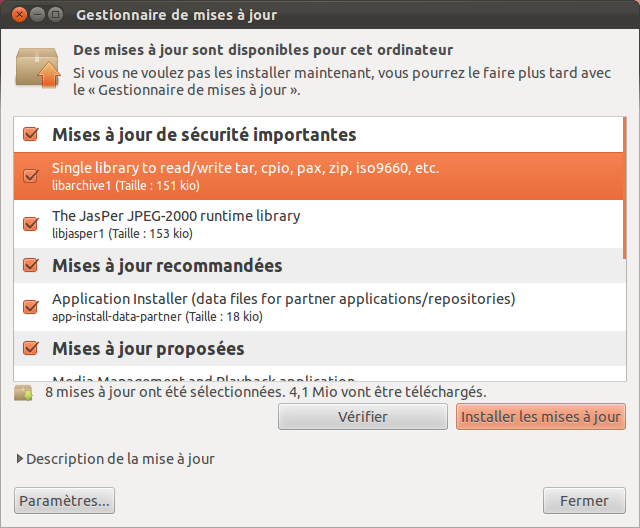
\includegraphics[scale=0.4] {./images/Maj02.png}
\end{center}
\end{frame}

%----------------------------------------------------------------------------------------
\begin{frame}
\frametitle{ Installation de logiciels}
\justifying{
\begin{block}{Logiciels payants - propriétaires}
\begin{itemize}
\item Pas de logiciels crackés
\item Pas de téléchargement de logiciels depuis un autre site que le site officiel.
On oublie les sites 01Net, Télécharger.com qui remplacent le navigateur par Chrome...
\item Que les logiciels dont on a besoin (pas de démos, de logiciels marrants...)
\end{itemize}
\end{block}

\begin{block}{Logiciels libres}
\begin{itemize}
\item Préférer le logiciel libre - open source.
\item Passer par l'annuaire de Framasoft.
\end{itemize}
\end{block}
}
\end{frame}

%----------------------------------------------------------------------------------------
\begin{frame}
\frametitle{ Le copain qui s'y connait}

\begin{block}{Attention}
\begin{itemize}
\justifying{
\item Ne pas le laisser installer les logiciels crackés.
\item Chercher à comprendre ce qu'il fait, lui demander. 
\item S'il n'est pas capable d'expliquer, se méfier. Voire refuser.
}
\end{itemize}
\end{block}

\begin{block}{PC = Personal Computer}
\begin{itemize}
\justifying{
\item Ne pas faire confiance. Il ne faut pas prêter sa machine sans voir ce que fait l’individu à qui vous l’avez confiée.
\item Il faut prévoir  une session invitée. 
\item Il est si facile d’installer un virus sur un PC... Méfiez-vous de ce que l'on fait sur votre PC.
}
\end{itemize}
\end{block}
\end{frame}

%----------------------------------------------------------------------------------------
\begin{frame}
\frametitle{Résumé}
\begin{columns}[c] 
\column{.55\textwidth} 
\begin{center}

\includegraphics[scale=0.8] {./images/gnu.jpg} 
\end{center}
\column{.5\textwidth} 
\begin{center}

\includegraphics[scale=0.8] {./images/linux.jpg} 
\end{center}
\end{columns}
\begin{block}{Bilan}
\begin{itemize}
\justifying{
\item Vous voulez éviter le gros de la contamination virale : GNU/Linux. 
\item Evitez les sites de Warez, de porno, les installations de logiciels piochés à gauche et à droite sur la toile, les clés USB.
\item De façon générale, lisez, apprenez, documentez-vous, ayez une utilisation rationnelle de votre ordinateur. 
 }
\end{itemize}
\end{block}
\end{frame}

%----------------------------------------------------------------------------------------
\begin{frame}
\begin{center}
\Huge{En appliquant, ces règles, on a tout de suite beaucoup moins de soucis avec son PC.}
\end{center}
\end{frame}


%========================================================================================
\begin{frame}
\begin{center}
\Huge{Hygiène numérique \& Internet}
\end{center}
\end{frame}

%----------------------------------------------------------------------------------------
\begin{frame}
\begin{center}
\Huge{Internet, quels principes}
\end{center}
\end{frame}

%----------------------------------------------------------------------------------------
\begin{frame}
\frametitle{Internet, un réseau de réseau}
\begin{itemize}
\justifying{
\item Internet c'est un réseau de réseau d'ordinateurs connectés entre eux.
\item Il y a les serveurs, des gros ordinateurs, sur lesquels il y a des sites Internet.
\item Il y a des routeurs, qui servent à transmettre les colis que l'on appelle "des paquets". 
\item Il y a la Box Internet qui est un point d'entrée de sortie sur Internet
\item Et enfin il y a notre ordinateur/tablette/smartphone...
}
\end{itemize}
\end{frame}

%----------------------------------------------------------------------------------------
\begin{frame}
\Huge{\centerline{Toutes ces traces qu'on laisse}}
\Huge{\centerline{sur Internet... sans le savoir}}
\end{frame}
\begin{frame}
\begin{center}
\Huge{Les données qui sont prises à notre insu...}
\\~\\
\Huge{Comment est-on suivi à la trace sur Internet?}
\end{center}
\end{frame}
%----------------------------------------------------------------------------------------
\begin{frame}
\frametitle{Comment est-on pisté ?}
\justifying{
\begin{block}{Toutes les publicités nous espionnent}
\begin{itemize}
\item Le bouton Like de Facebook : il permet à FaceBook de savoir que vous avez visité ce site, même si vous n'avez pas cliqué sur ce bouton.
\item Même si vous vous êtes correctement déconnecté de Facebook.
\item De même pour le bouton le +1 de Google, les scripts de Google Analytics, 
\item Tous les publicité, Amazon...
\end{itemize}
\end{block}
}
\begin{center}

\includegraphics[scale=0.3] {./images/Facebook_like.png}
\end{center}
\end{frame}

%----------------------------------------------------------------------------------------
\begin{frame}
\frametitle{Pour le voir, l'extension Lightbeam}
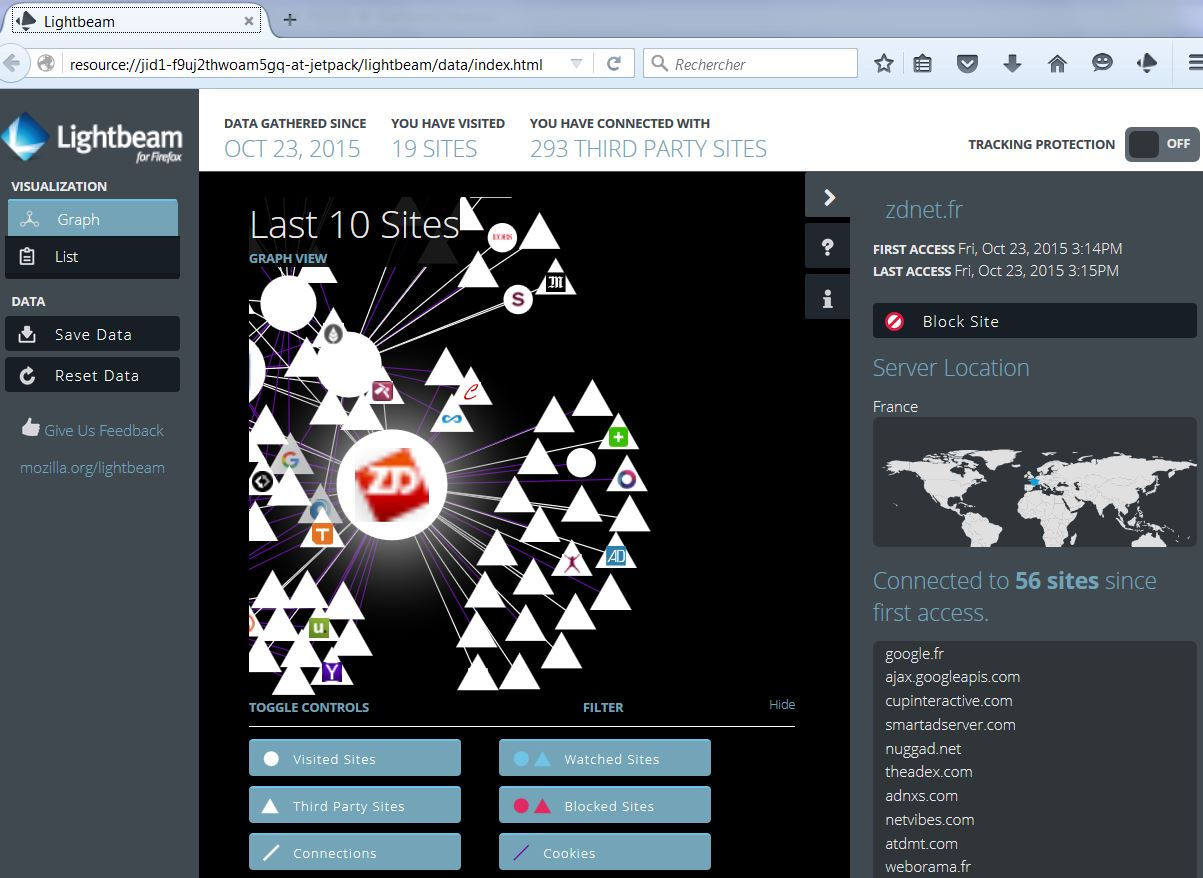
\includegraphics[scale=0.45] {./images/Lightbeam.jpg} 

\end{frame}

%----------------------------------------------------------------------------------------
\begin{frame}
\frametitle{Cloud - l'informatique dans les nuages}
\begin{block}{Définition du cloud}
\justifying{
\begin{itemize}
\item Le \emph{Cloud} , c'est l'ordinateur d'un autre.
\end{itemize}
}
\begin{center}

\includegraphics[scale=0.5] {./images/cloud.png} 
\end{center}
\end{block}
\end{frame}
%----------------------------------------------------------------------------------------

\begin{frame}
\begin{center}
\Huge{LES GAFAMs}\\~\\
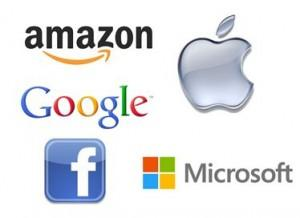
\includegraphics[scale=0.5] {./images/gafam.jpg} 
\end{center}
\end{frame}

%----------------------------------------------------------------------------------------
\begin{frame}
\frametitle{Les GAFAM}
\begin{block}{GAFAM : Google, Apple, Facebook, Amazon, Microsoft}
\begin{itemize}
\justifying{
\item Concentration des acteurs d’Internet autour de silos ;
\item Une centralisation nuisible (frein à l'innovation) ;
\item Les utilisateurs de ces services ne contrôlent plus leur vie numérique.
}
\end{itemize}
\end{block}
\end{frame}

%----------------------------------------------------------------------------------------
\begin{frame}
\begin{center}
\Huge{Sur Internet, si c'est gratuit, c'est VOUS le produit}
\end{center}
\end{frame}


%----------------------------------------------------------------------------------------
\begin{frame}
\begin{center}
\includegraphics[scale=0.65] {./images/couverture-livre-surveillance_m.jpg}
\end{center}
\end{frame}

\begin{frame}
\begin{center}
\Huge{Hygiène numérique \& Internet}
\end{center}
\end{frame}

%----------------------------------------------------------------------------------------
\begin{frame}
\frametitle{Choisir le bon navigateur}
\begin{center}
\includegraphics[scale=0.3] {./images/Firefox.jpg}
\end{center}
\end{frame}

%----------------------------------------------------------------------------------------
\begin{frame}
\frametitle{La navigation en mode privé 1/2}

\justifying{
\begin{block}{Quelles données ne sont pas enregistrées durant la navigation privée ?}
\begin{itemize}
\item pages visitées ;
\item saisies dans les formulaires et la barre de recherche ;
\item mots de passe ; 
\item liste des téléchargements ; 
\item cookies ;
\item fichiers temporaires ou tampons.
\end{itemize}
\end{block}
}
\end{frame}

%----------------------------------------------------------------------------------------
\begin{frame}
\frametitle{La navigation en mode privé 2/2}
\begin{center}
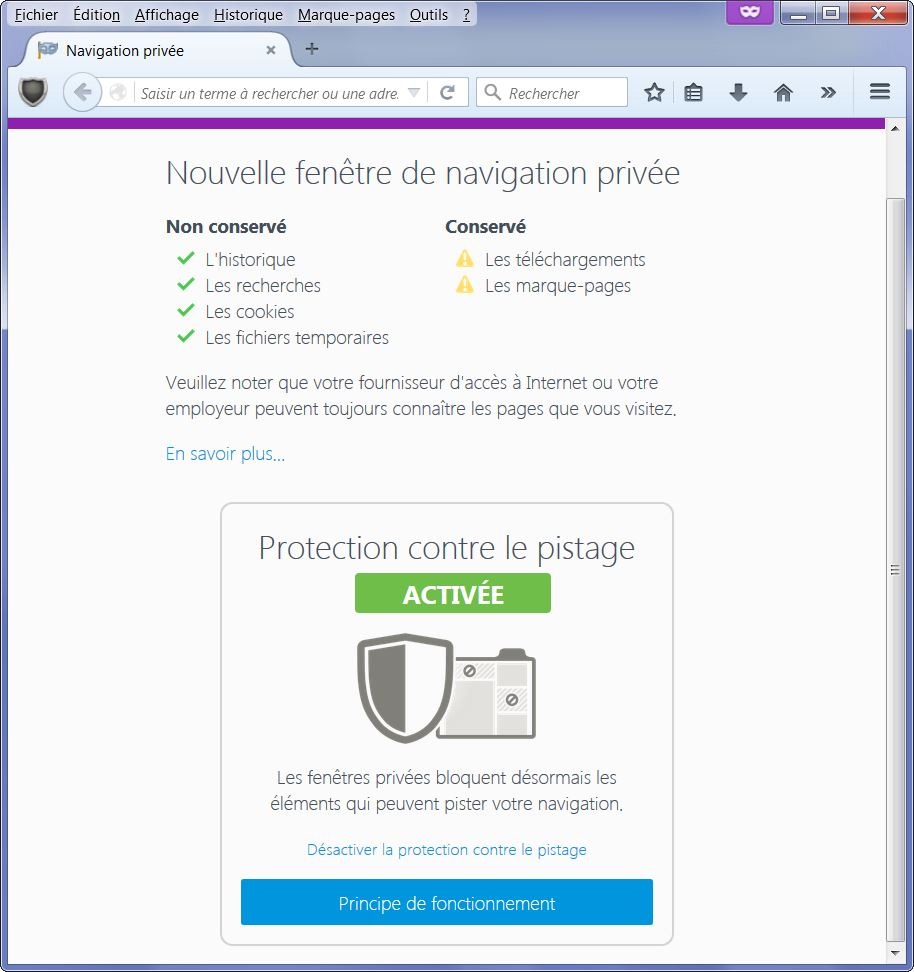
\includegraphics[scale=0.5] {./images/Navigation_privee.jpg} 
\end{center}
\end{frame}

%----------------------------------------------------------------------------------------
\begin{frame}
\frametitle{Installer des extensions}
\begin{center}
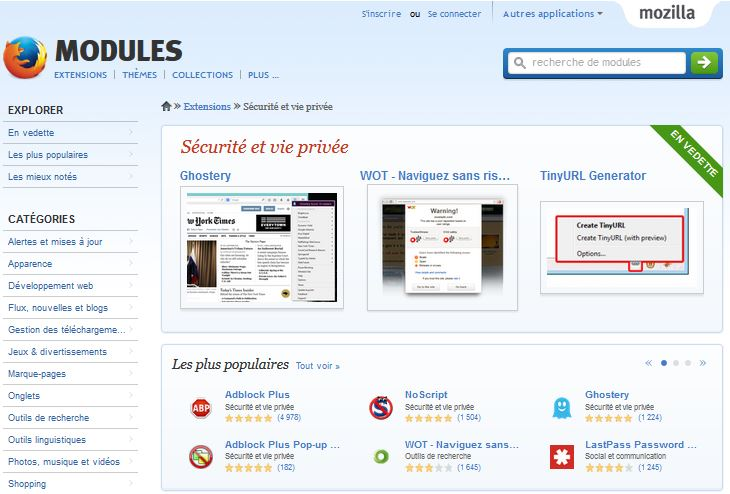
\includegraphics[scale=0.75] {./images/extensions_firefox.jpg}
\end{center}
\end{frame}

%----------------------------------------------------------------------------------------
\begin{frame}
\frametitle{Ublock Origins - Bloquer les publicités}
\begin{center}
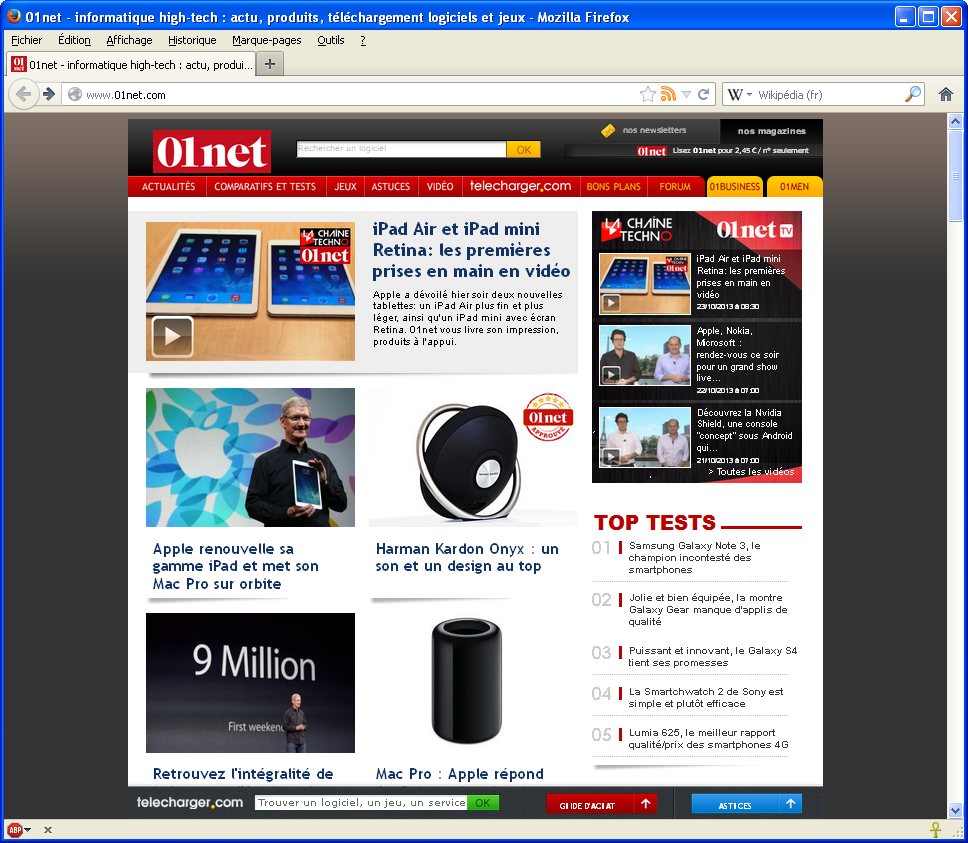
\includegraphics[scale=0.4] {./images/Adblock02.png}
\end{center}
\end{frame}

%----------------------------------------------------------------------------------------
\begin{frame}
\frametitle{Ghostery, Privacy Badger, Noscript...}
Bloquer tous les trackers associés au site.
\begin{center}
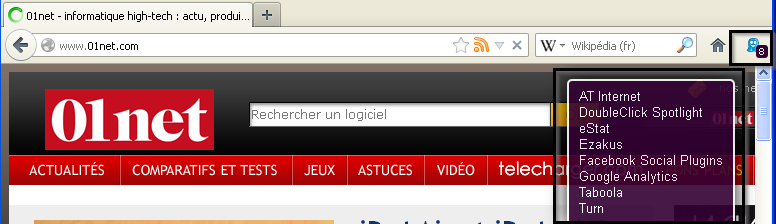
\includegraphics[scale=0.4] {./images/Ghostery_tracker.png}
\end{center}
\end{frame}

%----------------------------------------------------------------------------------------
\begin{frame}
\begin{center}
\Huge{Changer de moteur de recherche}
\\~\\
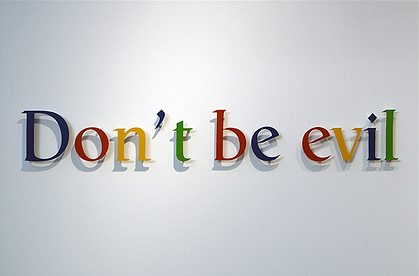
\includegraphics[scale=2] {./images/dontbeevil.jpg}
\end{center}
\end{frame}
%----------------------------------------------------------------------------------------
\begin{frame}
\begin{center}
\frametitle{Duckduckgo - Google tracks you. We don't.}

\url{https://duckduckgo.com}
\\~\\
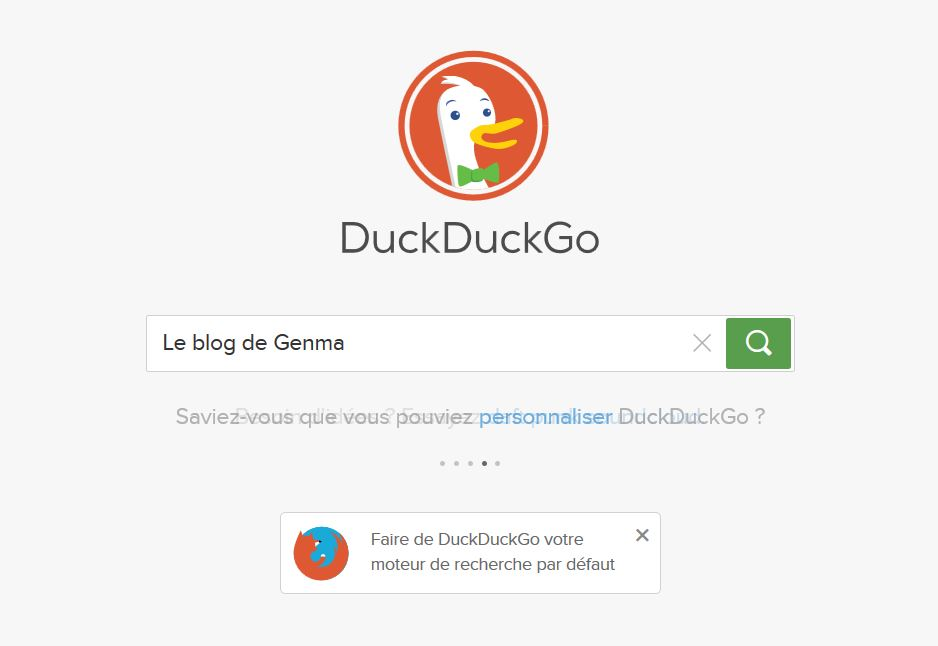
\includegraphics[scale=0.6] {./images/DuckDuckGo.jpg}
\end{center}
\end{frame}

\begin{frame}
\begin{center}
\frametitle{Par Framasoft}

Framabee \url{https://framabee.org} \\ou TontonRoger \url{https://tontonroger.org/}
\\~\\
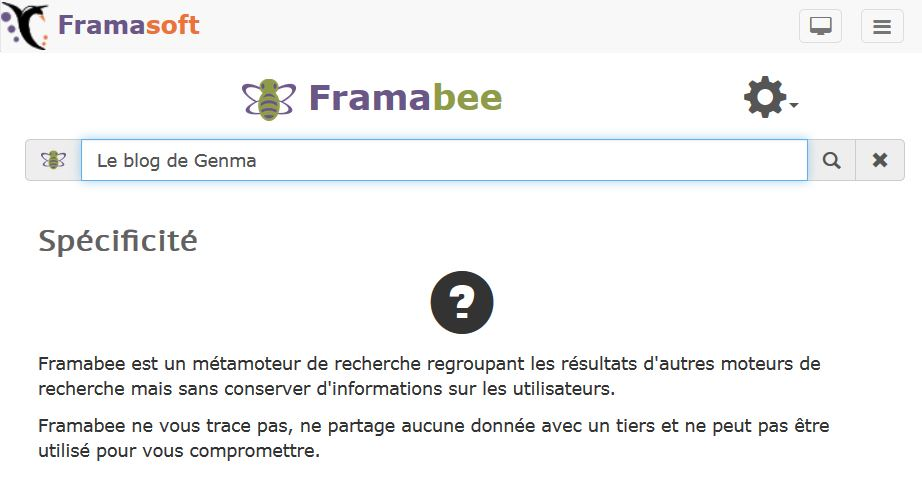
\includegraphics[scale=0.6] {./images/Framabee.jpg}
\end{center}
\end{frame}

\begin{frame}
\begin{center}
\frametitle{Qwant}

\url{https://qwant.com}
\\~\\

\includegraphics[scale=0.6] {./images/Qwant.jpg}
\end{center}
\end{frame}

%----------------------------------------------------------------------------------------
\begin{frame}
\begin{center}
\Huge{Changer de Cloud}
\\~\\
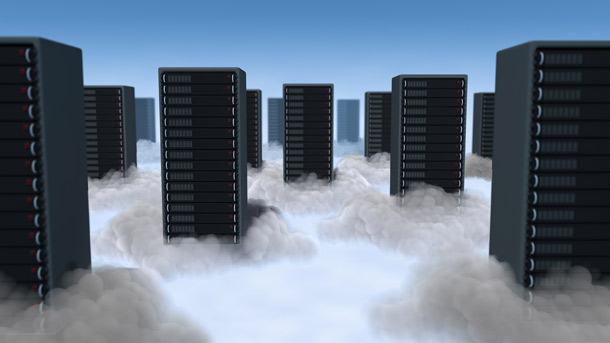
\includegraphics[scale=0.35] {./images/cloud_data_center.jpg}
\end{center}
\end{frame}

%----------------------------------------------------------------------------------------
\begin{frame}
\begin{center}
\frametitle{Framasoft et tous ses outils de Degooglisons}
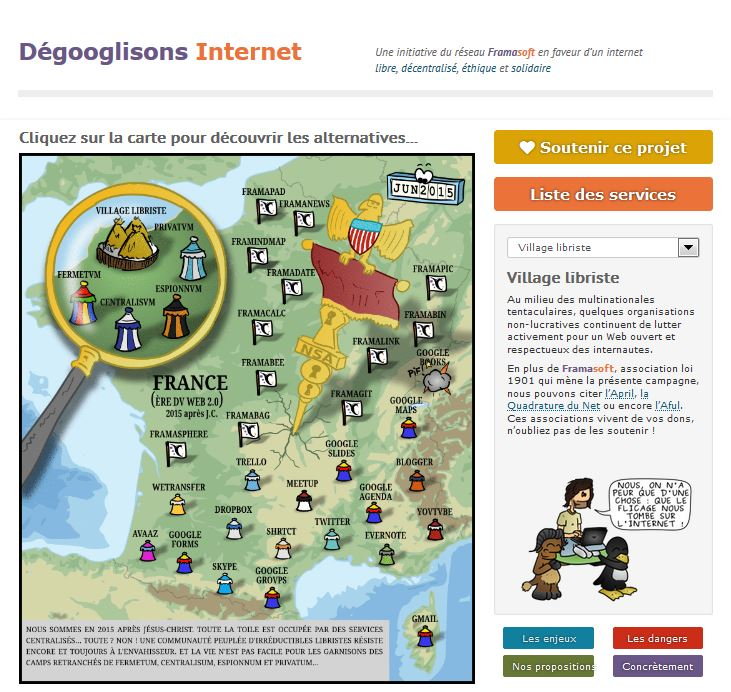
\includegraphics[scale=0.6] {./images/framasoft_degogglisons.jpg}
\end{center}
\end{frame}
%----------------------------------------------------------------------------------------
\begin{frame}
\begin{center}
\frametitle{Cozycloud}
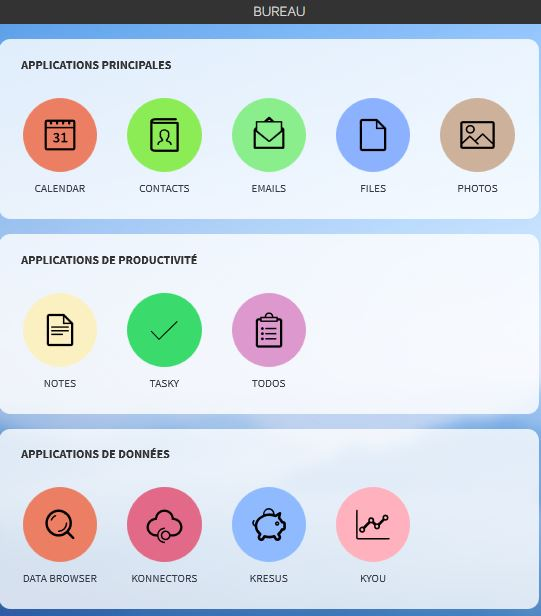
\includegraphics[scale=0.6] {./images/Cozycloud.jpg}
\end{center}
\end{frame}

%----------------------------------------------------------------------------------------
\begin{frame}
\begin{center}
\frametitle{Owncloud /NextCloud}
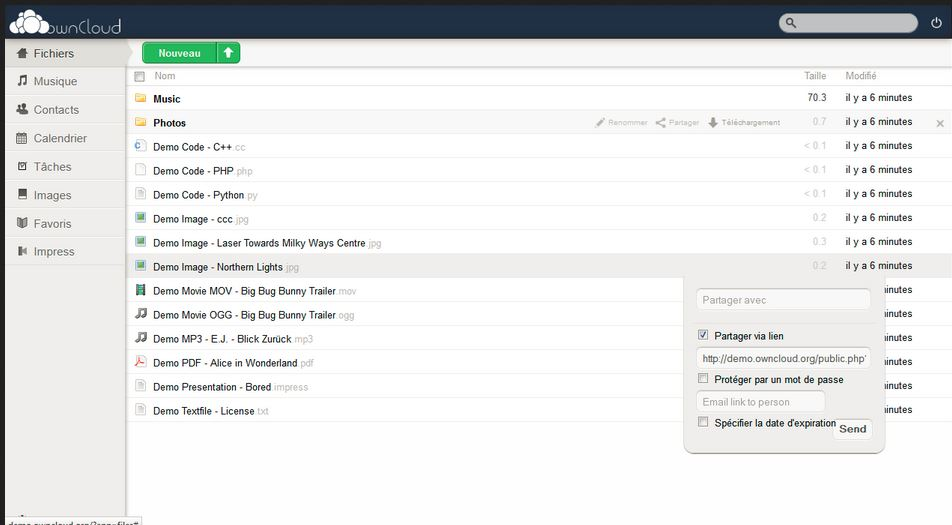
\includegraphics[scale=0.6] {./images/owncloud.jpg}
\end{center}
\end{frame}
%----------------------------------------------------------------------------------------
\begin{frame}
\begin{center}
\frametitle{La brique Internet}
\url{http://labriqueinter.net}
\\~\\
\includegraphics[scale=0.1] {./images/labriqueinternet.png}
\end{center}
\end{frame}

%----------------------------------------------------------------------------------------
\begin{frame}
\begin{center}
\frametitle{Yunohost}
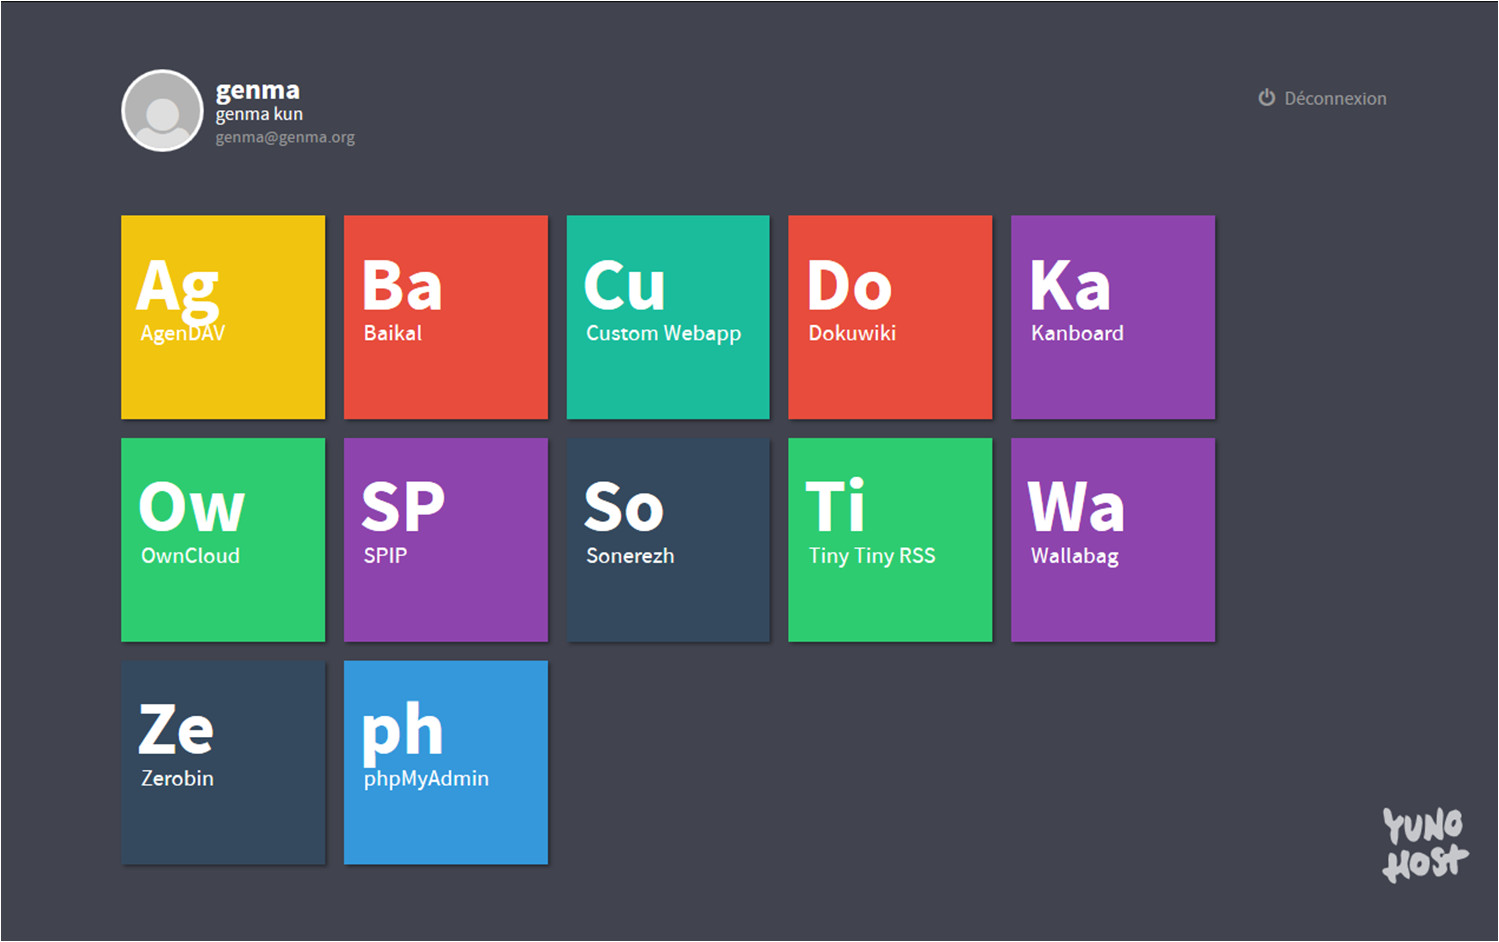
\includegraphics[scale=0.25] {./images/Yunohost.jpg}
\end{center}
\end{frame}

%-----------------------------------------------
\begin{frame}
\begin{center}
\Huge{Pour vous aider, \\~\\Le monde associatif}
\end{center}
\end{frame}

%-----------------------------------------------
\begin{frame}
\frametitle{Sur Paris - Parinux}

\begin{block}{Premier Samedi du Libre (PSL)}
\justifying{Chaque premier samedi de chaque mois, les bénévoles des associations du Libre vous accueillent au Carrefour Numérique de la Cité des sciences et de l'industrie (CSI) pour une install party.\\ \url{http://premier-samedi.org/}
}
\end{block}
\begin{center}

\includegraphics[scale=0.5] {./images/parinux.png}
\end{center} 
\end{frame}
%-----------------------------------------------
\begin{frame}
\frametitle{Ubuntu Party}
\begin{block}{Ubuntu-fr}
Ubuntu Party
\url{http://www.ubuntu-paris.org/}
\end{block}
\begin{center}
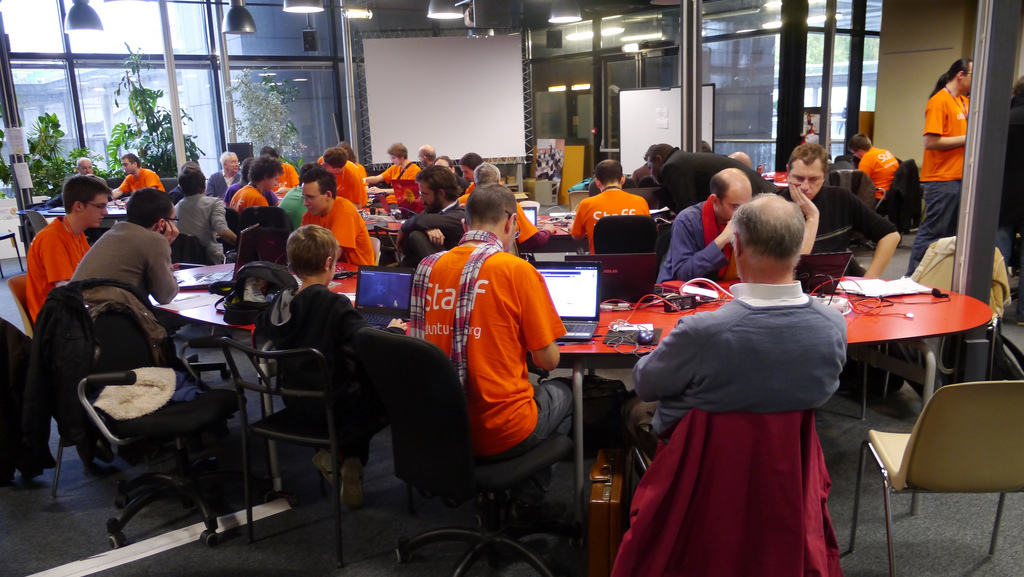
\includegraphics[scale=0.3] {./images/ubuntu-paris.jpg}
\end{center} 
\end{frame}
%-----------------------------------------------
\begin{frame}
\frametitle{Agenda du libre }
\begin{center}
\url{http://www.agendadulibre.org/}
\\
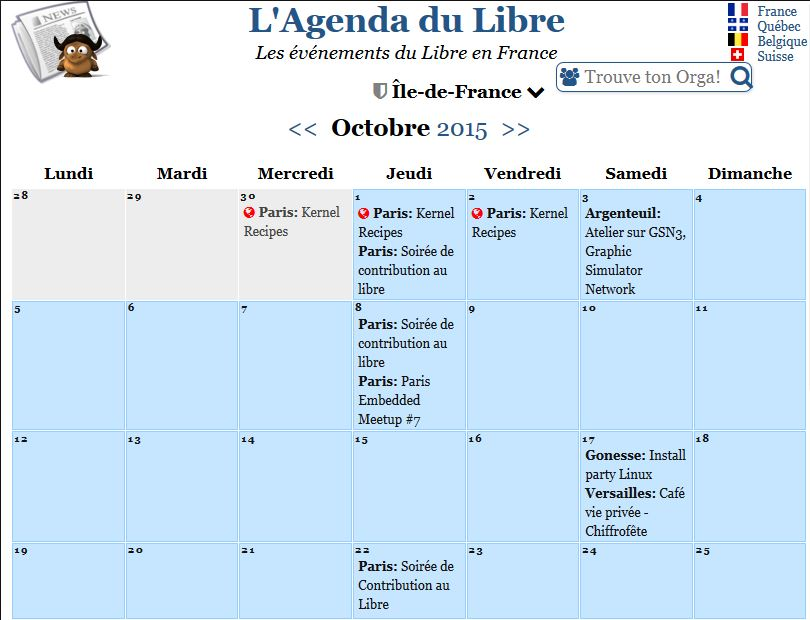
\includegraphics[scale=0.55] {./images/agenda-du-libre.jpg}
\end{center} 
\end{frame}

%----------------------------------------------------------------------------------------
\begin{frame}
\begin{center}
\Huge{Café vie privée, chiffrofête, cryptoparty}
\\~\\

\includegraphics[scale=0.3] {./images/LogoCafeViePrivee.jpg}
\end{center}
\end{frame}

\begin{frame}
\begin{center}
\Huge{Merci de votre attention}
\\
\Huge{Place aux questions.}
\\~\\
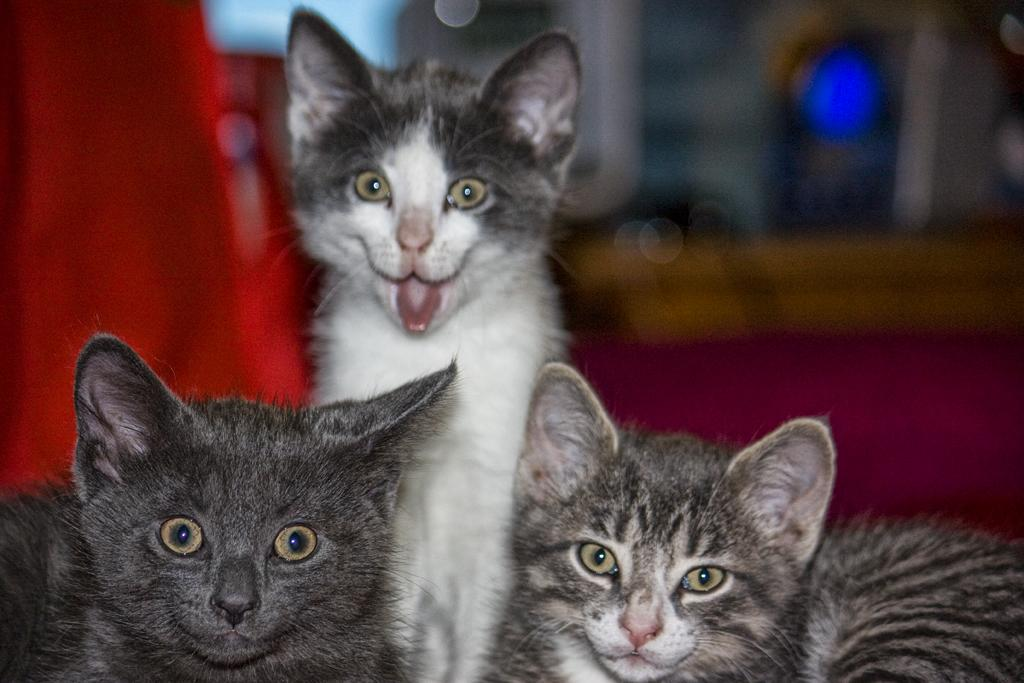
\includegraphics[scale=0.2] {./images/chat.jpg}
\end{center}
\end{frame}


%----------------------------------------------------------------------------------------
\begin{frame}
\frametitle{
\includegraphics[scale=0.4]{./images/Genma.jpg} \ \ \  Me contacter?}
\Huge{\centerline{Le Blog de Genma}}
\Huge{\centerline{https://blog.genma.fr}}
\Huge{\centerline{~}}
\Huge{\centerline{Twitter : @genma}}
\end{frame}


%========================================================================================
\begin{frame}
\begin{center}
\Huge{ANNEXES}
\end{center}
\end{frame}

%----------------------------------------------------------------------------------------
%----------------------------------------------------------------------------------------
\begin{frame}
\begin{center}
\Huge{Règles de sécurité supplémentaires}
\end{center}
\end{frame}
\begin{frame}
\Huge{\centerline{L'authentification forte}}
\end{frame}

\begin{frame}
\frametitle{L'authentification forte}
\begin{block}{Différents termes, un même usage}
Double authentification, Connexion en deux étapes, 2-Step Verification
\end{block}
\begin{block}{Exemple avec Google} 
\justifying{
Google permet aux utilisateurs d'utiliser un processus de vérification en deux étapes.
\begin{itemize}
\item La première étape consiste à se connecter en utilisant le nom d'utilisateur et mot de passe. Il s'agit d'une application du facteur de connaissance.
\item Au moment de la connexion Google envoit par SMS un nouveau code unique. Ce nombre doit être entré pour compléter le processus de connexion. 
\end{itemize}
Il y a aussi une application à installer qui génère un nouveau code toutes les 30 secondes.
}
\end{block}
\end{frame}

%----------------------------------------------------------------------------------------
\begin{frame}
\frametitle{L'authentification forte}
\begin{block}{Autres services implémentant cette fonctionnalité}
\begin{itemize}
\item Web : Facebook, Twitter, Linkedin, Paypal
\item Banque : envoi d'un code par SMS
\end{itemize}
\end{block}
\end{frame}

%------------------------------------------------
\begin{frame}
\frametitle{Comment vérifier rapidement la sécurité d'un site ?}
\begin{block}{La check-liste}
\begin{itemize}
\justifying{
\item Le site a-t-il une connexion en https ? (SSL).
\item Y-a-t-il intégration d'éléments extérieurs au site en lui-même ?
\item Le site utilise-t-il Google Analytics ?
\item Le site utilise-t-il Google Fonts ?
\item Le site utilise-t-il des régies publicitaires ?
\item Le site utilise-t-il Cloudflare ?
\item Le DNS est-il géré par Cloudflare ?
\item Le site présente-t-il une politique de confidentialité ?
\item Le site utilise-t-il les cookies ?
\item Le site utilise-t-il des scripts javascript ?
}
\end{itemize}
\end{block}
\end{frame}

%----------------------------------------------------------------------------------------
%----------------------------------------------------------------------------------------
\begin{frame}
\begin{center}
\Huge{httpS}
\end{center}
\end{frame}
%----------------------------------------------------------------------------------------

\begin{frame}
\frametitle{HTTPSEverywhere}
Force le passage en https quand celui-ci est proposé par le site.
\begin{center}
\includegraphics[scale=0.4] {./images/https-everywhere.jpg}
\end{center}
\end{frame}

%----------------------------------------------------------------------------------------
\begin{frame}
\frametitle{HTTPSEverywhere}
\begin{center}
\includegraphics[scale=0.4] {./images/Https_SSL_Observatory.jpg}
\end{center}
\end{frame}

%----------------------------------------------------------------------------------------
\begin{frame}
\frametitle{Certificate Patrol}
Permet de valider les certificats d'un site (lié à https).
\begin{center}
\includegraphics[scale=0.5] {./images/CertificatePatrol.png}
\end{center}
\end{frame}

%----------------------------------------------------------------------------------------
\begin{frame}
\frametitle{Certificate Patrol}
\begin{center}
\includegraphics[scale=0.5] {./images/Certificate_Patrol_certifcat_a_change.jpg}
\end{center}
\end{frame}

%----------------------------------------------------------------------------------------
\begin{frame}
\frametitle{Calomel SSL}
\begin{center}
\includegraphics[scale=0.5] {./images/Calomel.jpg}
\end{center}
\end{frame}

%----------------------------------------------------------------------------------------
%----------------------------------------------------------------------------------------
\begin{frame}
\begin{center}
\Huge{Utilisation d'Internet \\depuis un lieu public}
\end{center}
\end{frame}

%----------------------------------------------------------------------------------------
\begin{frame}
\frametitle{Utilisation d'un PC d'un Cybercafé?}

\begin{block}{Pour le surf Internet}
\begin{itemize}
\justifying{
\item Eviter les sites sur lesquels on sait des données personnelles : webmail, réseaux sociaux
\item Vérifier la version du navigateur
\item  Ne pas mémoriser vos informations confidentielles
\item  Penser à fermer votre session
\item  Effacer vos traces de navigation
}
\end{itemize}
\end{block}
\justifying{
Ne pas brancher de clef USB (virus), ne pas récupérer de documents.
\\
Idéalement ? Un navigateur en mode portable, depuis une clef USB
\\
Encore mieux : rebooter sur un live-usb/cd
}
\end{frame}
%----------------------------------------------------------------------------------------
\begin{frame}
\frametitle{Wi-Fi public?}
Ne pas avoir confiance. Utiliser sa propre machine.
\begin{block}{Attention à la sécurisation}
\begin{itemize}
\justifying{
\item Au minimum : connexion HTTPS
\item Mieux, passer par un VPN
}
\end{itemize}
\end{block}
\end{frame}

%----------------------------------------------------------------------------------------
%----------------------------------------------------------------------------------------
\begin{frame}
\begin{center}
\Huge{Internet \& Surveillance}
\end{center}
\end{frame}
%----------------------------------------------------------------------------------------
\begin{frame}
\begin{center}
\includegraphics[scale=0.5] {./images/nothingtohide.png} 
\end{center}
\end{frame}

\begin{frame}
\frametitle{L'espionnage 1/2}
\begin{center}
\includegraphics[scale=0.4]{./images/snowden.png}
\end{center}
\begin{itemize}
\item Snowden et ses révélations (NSA)
\item La loi Renseignement en France…
\end{itemize}
\end{frame}

\begin{frame}
\frametitle{L'espionnage 2/2}
\begin{itemize}
\item Notre voisin
\item Notre "ex"
\item Notre collègue de boulot 
\end{itemize}
\includegraphics[scale=0.55]{./images/nixon.jpg}
\includegraphics[scale=0.4]{./images/girlfriend.jpg}
\end{frame}

\begin{frame}
\frametitle{La différence entre la vie privée et la sécurité en une image}
\begin{center}
\includegraphics[scale=0.4]{./images/Security_Privacy.jpg}
\end{center}
\end{frame}

\begin{frame}
\frametitle{Différents \emph{modèles de menace}}
\begin{block}{Répondre aux questions}
\justifying{
Pour se faire un avis \url{http://jenairienacacher.fr/}
\begin{itemize}
\justifying{
\item Quelles sont les données et informations que j'estime personnelles - confidentielles? 
\item Qu'est ce que je suis prêt-e à apprendre et à faire pour les protéger?
\item Usage d'un pseudonyme...
}
\end{itemize}
}
\end{block}

\begin{center}
\includegraphics[scale=0.4]{./images/bannierepseudonymat.jpg}
\end{center}
\end{frame}
%----------------------------------------------------------------------------------------
\end{document}
